\documentclass[12pt]{article}
\usepackage[hmargin=1in,vmargin=1in,includefoot]{geometry} 
\usepackage{braket}
\usepackage{pgfgantt}
\usepackage{tikz}
\usepackage{relsize}
\usepackage{graphicx}% Include figure files
\usepackage{enumitem} %enumerate with letters, etc
\usepackage{float} %to better place figures
\usepackage{amsmath}
\usepackage{amsthm}
\usepackage{amssymb}
\usepackage{bm}
\usepackage{wrapfig}
%\usepackage{setspace}
%\doublespacing

\usetikzlibrary{tikzmark,fit,shapes.geometric}
\usetikzlibrary{arrows,shapes,positioning}
\usetikzlibrary{decorations.markings}

\definecolor{darkred}{RGB}{128,0,0}
\definecolor{palegoldenrod}{RGB}{238,232,170}

\tikzstyle arrowstyle=[scale=1]

\tikzstyle directed=[postaction={decorate,decoration={markings,mark=at position .5 with {\arrow[arrowstyle]{stealth}}}}]
\tikzstyle reverse directed=[postaction={decorate,decoration={markings, mark=at position .5 with {\arrowreversed[arrowstyle]{stealth};}}}]

\usepackage{mathtools}
\mathtoolsset{showonlyrefs}
%\pagenumbering{gobble}

\makeatletter
\def\@maketitle{%
  \newpage
  \vspace*{-\topskip}      % remove the initial space
  \begingroup\centering    % instead of \begin{center}
  \let \footnote \thanks
  \hrule height \z@        % to avoid the insertion of lineskip glue
    {\LARGE \@title \par}%
    \vskip 1.5em
    {\large
      \lineskip .5em
      \begin{tabular}[t]{c}%
        \@author
      \end{tabular}\par}%
  \par\endgroup            % instead of \end{center}
  \vskip 1.5em             % <--- modify this to adjust the separation
}
\makeatother

\begin{document}

\title{Forging new pathways to improved nuclear-reaction predictions}
\author{PI: Mack Atkinson (PLS/NACS, Postdoc, 50\%) \\
Cole Pruitt (WCI 10\%) \\
Gregory Potel (PLS/NACS, 10\%) \\
Sofia Quaglioni (PLS/NACS, 5\%) \\
Willem Dickhoff (Washington University in St. Louis, unpaid) \\
Kazuki Yoshida (Japan Atomic Energy Agency, unpaid)
}
\maketitle


\vspace{4cm}
\textbf{Executive Summary} - Here goes the executive summary (2 sentences)

\vspace{2cm}
\textbf{Plain Language Description} - Paragraph describing proposal

\newpage

%\section{Introduction}
%The origin and abundance of all atomic nuclei lies at the heart of nuclear physics.
\textcolor{blue}{\textbf{Introduction}}
 %- How do neutrons and protons arrange themselves to produce stable atomic nuclei and rare isotopes?    
 - Almost everything that is known in nuclear physics today has been learned from reactions of nuclei with external probes (e.g.
 electrons and photons) and nuclear probes. The motivation for decades of nuclear-reaction experiments can be expressed
 with a single question - how do neutrons and protons arrange themselves to produce stable atomic nuclei and rare
 isotopes? This intriguing and yet basic question is at the heart of nuclear structure research - the study of the
 properties of atomic nuclei in isolation such as nuclear masses and sizes, characteristic energy levels, and
 radioactive decay modes.
Depending on the proton-neutron imbalance and excitation energy, nucleons can display single-particle behavior giving
rise to a shell structure picture of nuclei (analagous to electronic shell structure in atoms) but can also organize
into distinct ``cluster" substructures or even move coherently producing collective oscillatory, rotational, and/or
vibrational modes.
While nuclear structure models do a remarkable job describing stable nuclei, they diverge from reality when considering nuclei
away from stability (nuclei with excess neutrons or excess protons). To reach a better understanding of these
exotic nuclei, we once again rely on nuclear reactions.

%By inducing reactions of nuclei with either external probes (electrons, photons, etc.) or nuclear probes, 
%Much progress has been made by investigating the nature of atomic nuclei through nuclear scattering
%experiments. 


Traditionally, isotopes are studied by impinging a target comprised of the
given isotope with a projectile beam (electrons, protons, etc.). In particular, electron scattering provides the
cleanest way to extract nuclear structure properties owing to the perturbative nature of the EM interaction. Unstable
(or rare) isotopes, however, are too short-lived to form into a target and instead are studied through an inverse
process where the beam itself is comprised of the rare isotope which is impinged on a target of stable nuclei.  The
DOE's flagship facility for nuclear science, the Facility for Rare Isotope Beams (FRIB), which started user operations
in May 2022, produces beams of rare isotopes to be studied in this inverse process.  
FRIB enables us to study the structure rare isotopes away from stability to improve nuclear structure models. 
However, these capabilities at
FRIB can only be fully utilized if there is a suitable reaction theory that links nuclear structure to the reaction
observations. 
%However, the path toward understanding nuclei at the limits of stability not only includes the construction of world-class experimental
%facilities, but simultaneously 
Thus, the path toward understanding nuclei at the limits of stability is the unified,
simultaneous development and communication between three areas: improved experimental techniques and facilities to measure
unstable nuclei (i.e. FRIB), the development of more precise nuclear structure models, and the development of better reaction
theories.
With this in mind, the aim of our project is to provide more accurate reaction calculations.

%While electron scattering provides the cleanest way to extract nuclear structure
%properties of stable nuclei owing to the perturbative nature of the electromagnetic interactions, rare isotopes can only
%be studied in the nucleus-nucleus collisions induced at facilities like FRIB. 
%%Since the advent of nuclear physics, scientists have studied isotopes through scattering experiments. 
%Because nuclei away from stablity are short-lived, they cannot be used as targets for traditional scattering techniques such as
%electron scattering (which provides a clean way to extract nuclear structure properties owing to the perturbative nature
%of the EM interaction).  
%Nuclear scattering experiments often (involving the collision of a given isotope) 
%In order to study these short-lived rare isotopes, 
%The study of these rare isotopes is now possible thanks to the DOE's flagship facility for nuclear science, the Facility
%for Rare Isotope Beams (FRIB), which started user operations in May 2022. FRIB can generate rare isotope beams which can
%be collided with 

 %This fundamental question has been the underlying motivation in the advancement of nuclear physics
 %for over half a century now. After all this time, even with all the discoveries and advancements in the field, we still don't have the answer to this simple question. 
%Much
 %progress has been made toward an answer by investigating the nature of atomic nuclei through nuclear scattering experiments. 
 %%By observing (and quantifying) the collision of
 %%nuclei, the mechanisms that dictate the subsequent motion of nucleons (protons or neutrons) can be unravelled. 
%%The way in which nuclei respond in nuclear reactions helps to inform the nature of the nuclear force - the underlying interaction between neutrons and protons that governs the
%%formation of nuclei. 
 %To reach a fundamental understanding of nuclei, a suitable reaction theory is vital in order to interperet experimental
 %data. 
 %%Experimental techniques, instruments, and facilities are advancing at a rapid rate, so nuclear reaction theory must
 %%progress in tandem.
 %A looming challenge in nuclear reaction theory is to provide state-of-the-art predictions for
 %the wealth of experimental data now being produced at DOE's flagship facility for nuclear science, the Facility for Rare Isotope Beams (FRIB), which started user operations in May
 %2022. FRIB is a facility that generates high-energy rare (unstable, exotic) isotope beams which allows for the study of these short-lived nuclei
 %which otherwise could not be studied (since they are too short lived to act as targets). This exploration of nuclei approaching the limits of
 %stability will provide new insights into the fundamental nuclear force as well as strengthen the nuclear data libraries underpinning energy and security applications. 
   %The evolution of nuclear structure as we approach the limits of stability is an overarching theme of the recent DOE Town Hall Meeting
 %which will determine the 2023 Nuclear Long Range Plan.
 %%In the 2015 Long Range Plan,
 %%it was said that "Scientific discoveries are often made by investigating nature at the extremes", which indeed explains the excitement of the nuclear community for FRIB science. 
   %Indeed, from the 2012 Decadal study of Nuclear Physics by the National Academies of Sience, "Nuclear Physics: Exploring the
 %Heart of Matter", it was said that, "Many of today’s most important advancements in medicine, materials, energy, security, climatology, and dozens of other sciences emanate from
 %the wellspring of basic research and development in nuclear physics. Answers to some of the most important questions facing our planet will come from nuclear science,
 %interdisciplinary efforts in energy and climate, and marketplace innovations". It is these observations that motivate our proposal to develop more complete reaction descriptions.
 %%that will help to propel our understanding of nuclear physics to the limits of stability.  
 %%interdisciplinary efforts in energy and climate, and marketplace innovations". It is these observations that motivate our pursuit of more complete reaction descriptions that will
 %%help to propel our understanding of nuclear physics to the limits of stability.  
 %%Our proposal is designed to aid in this pursuit contribute to the scientific community's investigations into nuclear structure by developing better predictions of nuclear reactions so that data from
 %%advanced experimental facilities can be fully utilized.
%%Thus, the main drive of this proposal is to develop a better pathway toward describing nuclear reactions so that the experimental data coming from these billion-dollar
 %%facilities can be optimally utilized.

%The first big step toward understanding the structure of atomic nuclei (that is, the way in which neutrons and protons
%arrange themselves inside the nucleus) was the advent of the nuclear shell model by Maria Goeppert Mayer in 1948 [CITE].
%While this elegant model does a remarkable job describing stable nuclei, it diverges from reality when considering nuclei
%away from stability (nuclei with excess neutrons or excess protons). Indeed, a rich set of interesting features start to
%appear for these exotic nuclei (such as halo clustering, shape coexistence, deformations) that the independent shell model
%has no way of describing. These exotic phenonema can be investigated through the scattering of rare isotopes (of which many
%systems were not possible to study before FRIB). However, connecting this rich nuclear structure to the experimental data is
%no easy task. In order to bridge the gap between scattering data and nuclear structure, structure-aware nuclear reaction
%theories have been developed. Thus, the path toward understanding nuclei at the limits of stability is the unified,
%simultaneous development and communication between three areas: improved experimental techniques and facilities to measure
%unstable nuclei (i.e. FRIB), the development of more precise nuclear structure models, and the development of better reaction
%theories. 

%I have identified
%an area where nuclear reaction theory can be improved, and thus this proposal is to improve reaction descriptions such that nuclear structure can more reliably be extracted from
%nuclear scattering data.

\begin{wrapfigure}{r}{0.5\textwidth}
   \label{fig:eep_p2p}
   \begin{center}
      \vspace{-1.0cm}
      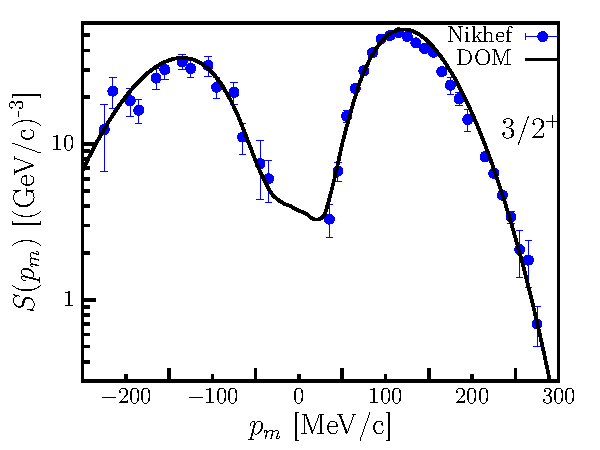
\includegraphics[width=0.49\linewidth]{figures/eep100.pdf}
      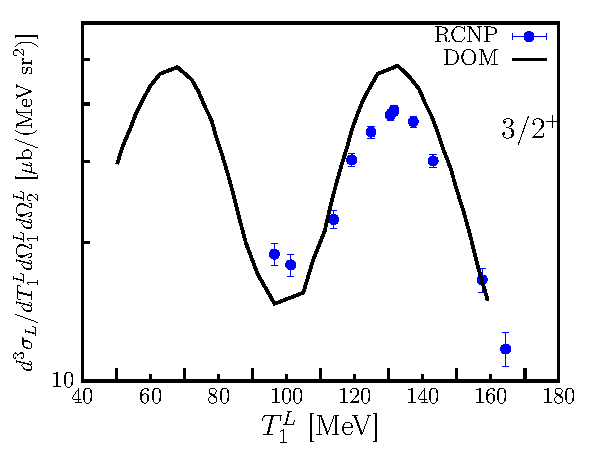
\includegraphics[width=0.49\linewidth]{figures/p2p.pdf}
      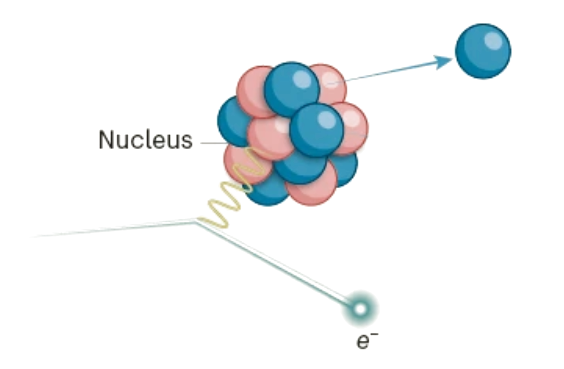
\includegraphics[width=0.49\linewidth]{figures/eep-schematic-alpha.png}
      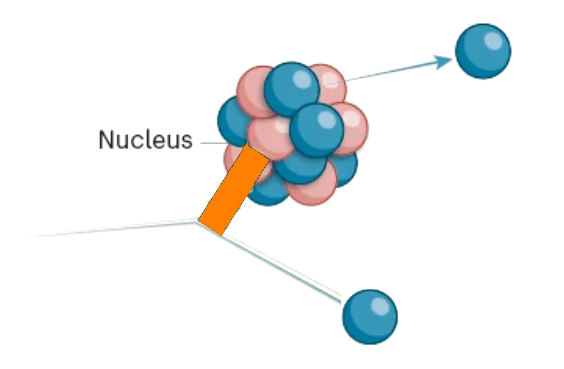
\includegraphics[width=0.49\linewidth]{figures/p2p-schematic-alpha_oldV.png}
      \vspace{-1.3cm}
   \end{center}
   \caption{A comparison of two knockout reactions, the left being induced by electrons and the right induced by protons.}
   %\caption{The left figure shows the results of a DWIA calculation of $^{40}$Ca$(e,e'p)^{39}$K using DOM ingredients. The right figure shows a similar DWIA calculation, except the
   %probe is now a proton rather than an electron, $^{40}$Ca$(p,2p)^{39}$K. While the same DOM ingredients are used in both cases, the electron-induced knockout reaction [left] reproduces
%the experimental data much more accurately than the proton-induced knockout reaction [right]. Below each curve is a schematic of each process.}
      \vspace{-0.5cm}
\end{wrapfigure} 
Especially useful are nucleus-induced reactions that remove a proton from a nucleus, denoted as $(p,2p)$, as they
provide a glimpse into how the removed proton arranged itself while it was in the nucleus. However, the theoretical
calculations of $(p,2p)$ reactions are currently not accurate enough to reliably extract this information. This is
demonstrated by the different outcome for the $(p,2p)$ and it's electron-induced counterpart $(e,e'p)$ reaction
calculations (see Fig.~\ref{fig:eep_p2p}).
%Our approach to improving nuclear-reaction calculations is to develop an effective nucleon-nucleon interaction that
%incorporates the effect of the nuclear medium. The need for an effective interaction is most clearly demonstrated
%in so-called knockout reactions where a projectile is used to knockout one or more protons (or neutrons) from a nucleus. 
%Employing a dispersive optical model (DOM), developed
%recently in the PI's PhD, the PI previously performed reaction calculations of both electron-induced knockout $(e,e'p)$ and proton-induced knockout $(p,2p)$ from the same nucleus
%$^{40}$Ca.  
The theoretical calculations of these two knockout reactions combine the same structure information from
$^{40}$Ca, all of which is consistently provided by the dispersive optical model (DOM) - a phenomenological model
developed by the PI during his PhD which leverages experimental data and Green's function theory to provide a robust
picture of the nucleus. The only difference between the two
calculations is the interaction between the probe (electron or proton) and $^{40}$Ca (see the bottom two schematics in
Fig.~\ref{fig:eep_p2p}). Even though most of the ingredients are the same in these two calculations, 
the electron-induced calculation follows the experimental data while the proton-induced calculation reveals a 20\%
discrepancy.
%there is a clear
%difference in the results when confronted with experimental data (see the top left and right panels in
%Fig.~\ref{fig:eep_p2p}). 
%Until now, there was not a model like the DOM that could provide the same, consistent
%ingredients to these reaction calculations. 
With only one difference between the two calculations, it is clear that the
deficiency is rooted in the interaction between the probing proton and $^{40}$Ca. The problem stems from the fact that the medium of the target is not taken into account when
employing the typical $pp$ interaction in $(p,2p)$ calculations. An attempt to include in-medium effects was made (with moderate success) over two decades ago by approximating the nucleus with infinite
nuclear matter (an idealized nuclear system) [CITE]. Since then, the $pp$ interaction used in $(p,2p)$ reactions has not seen development.
Building upon the state-of-the-art DOM, we will develop a new capability to accurately include the effect of the target medium into the $pp$ interaction, thus improving the
the accuracy of $(p,2p)$ reaction calculations.

%We plan to calculate 
%To rectify the deficiency, we will improve the proton-proton interaction causing the
%issue. By combinine elements in many-body theory with the DOM, we will generate a more realisting proton-proton interaction -
%an essential tool for interpreting reactions on unstable nuclei. 
%\begin{figure}[h]
   %\begin{tikzpicture}[node distance = 0.5cm]
      %\node[fill=green,dashed,rectangle,thick,draw,opacity=0.2,text opacity = 1] (a) at (0.2,0) 
      %{\begin{tikzpicture}
         %\node[align=center,ellipse,thick,draw,solid] (b) at (-1.6,0.5) { DOM \\ 
\includegraphics[scale=0.15]{figures/nucleus.png}};
         %\node[fill=orange,rectangle,thick,draw,solid,minimum width=0.15\linewidth] (c) at (1.7,0.5) {\small Old V};
         %\node[ellipse,thick,draw,solid] (d) at (0,-1) {\small Formalism};
         %\draw[solid] (b) -- (c);
         %\draw[solid] (c) -- (d);
         %\draw[solid] (b) -- (d);
      %\end{tikzpicture}
   %};
   %\node[rectangle,left=of a] (a2) {=};
   %\node[fill=green,rectangle,thick,draw,minimum width=0.15\linewidth,left=of a2] (a3) {\small New V};
   %\node[rectangle,right=of a] (b1) {$\implies$};
   %\node[rectangle] (b2) at (7,0) {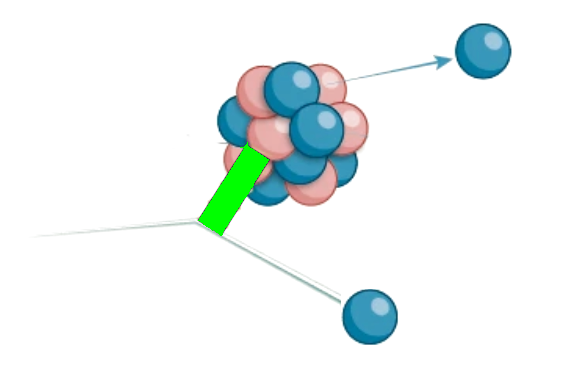
\includegraphics[scale=0.25]{figures/p2p-schematic-alpha_newV.png}};
         %%\node[rectangle,right=of b1] (b2) at (1,0) {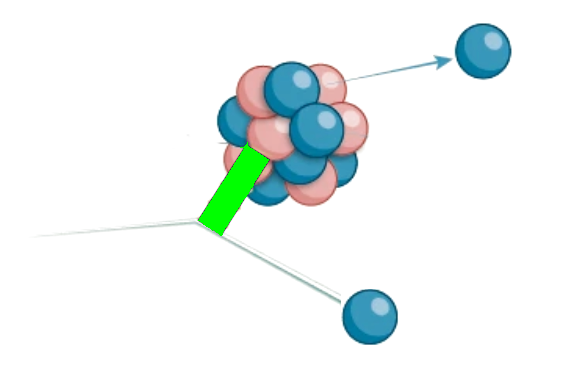
\includegraphics[scale=0.25]{figures/p2p-schematic-alpha_newV.png}};
%\end{tikzpicture}
%\caption{Schematic of the how the effective interaction is generated and how it is used to improve the proton-induced knockout reaction}
%\label{fig:schematic}
   %\end{figure}
%Until the DOM was developed, previous calculations of (p,2p) were always scaled to match the experimental data - meaning that there was no way to tell if there were a discrepancy
%in the structure description. Because of this, the proton-proton interaction used in the (p,2p) reaction has not seen development for over two decades. The most recent development
%was in 2000[CITE] where a group from Melbourne used infinite nuclear matter (an idealized nuclear system) in order to include some kind of nuclear-medium effects. Our implementation will
%be the first to actually include effects from finite nuclei in the effective interaction implemented in the proton-induced reaction. It may seem that a simpler solution to the
%difficulties of proton-induced reactions is to focus on electron-induced reactions since they pose less issues. The problem with electron-induced reactions it they require a stable
%target, and we (as a scientific community) are interested in the structure of nuclei near the limits of stability. As we mentioned earlier, unstable nuclei can only be studied with
%rare isotope beams like those generated at FRIB. Thus, we are working toward improving proton-induced (and more generally nucleon-induced) nuclear reactions through the development
%of an effective nucleon-nucleon interaction - an improvement that could account for discrepancies of roughly 20\%. 

\textcolor{blue}{\textbf{Project Plan}}
 - To develop a finite-nucleus-informed $pp$ and $pn$ interaction for nuclear reactions we consider the many ways in which a nucleon interacts as it propagates through a
nucleus. 
The formalism of Green's functions provides a natural framework for this task. Within it, one can compute the Green's function - or single-particle propagator - that specifies the
probability amplitude for a nucleon to travel from one place to another (within a nucleus) in a given period of time. The PI computed an accurate single-particle propagator during
his Ph.D. using the DOM. 
%A natural language to discuss this is the through Green's functions (or single-particle propagators) and perturbation theory~\cite{Exposed!}. Indeed, knowing the
%single-particle propagator of a nucleus is a powerful lever-arm in perturbation theory. We already have an accurate single-particle propagator from the DOM. 
With this, we have the
basic building-block to construct the dressed $pp$ and $pn$ interactions through the so-called ``ladder" approximation~\cite{Exposed!}. 
%By combining a bare nucleon-nucleon interaction and the DOM single-particle propagator, the effective interaction can
%be calculated using already-derived many-body formalism.   
   %The approximation that we can implement will be valid at energies approximately greater than 70 MeV/u, which also corresponds to the region of validity for the DWIA reaction
   %description of (p,2p).  

   
While the many-body formalism of the ladder approximation to an effective interaction has been known for some time now, it has only
been possible to implement in the fictional system of infinite nuclear matter [CITE]. The limitation, until now, has been
obtaining an accurate single-particle propagator for finite nuclei. Now that the DOM provides the single-particle propagator
in finite nuclei, we can apply this formalism in a realistic system. 
While this ladder approximation
will be implemented in a general way, we will specifically be calculating the dressed $pp$ and $pn$ interactions in $^{40}$Ca. 

%Implementing the many-body formalism in a finite system
%is still nontrivial however, even starting from an already-known propagator. The largest bottle neck in the computation of
%this interaction will be a large matrix inversion. Not only will the matrix inversion be computationally costly, but the
%generation of the matrix involves multi-dimensional integrals which will be computationally demanding. 
%While this many-body
%formalism will be implemented in a general way, we will specifically be calculating the effective interaction in $^{40}$Ca as
%it is a doubly-magic nucleus and the DOM describes it well. Generally, our objectives are to generate this effective
%interaction while demonstrating how it enhances reaction calculations through some specific cases:
\\
\textbf{Objective I: Calculate the effective interaction in $^{40}$Ca}
I will combine a chiral NN interaction (the ones typically used in \textit{ab initio} calculations [CITE]) with the DOM
proton propagator of $^{40}$Ca to generate an effective proton-proton interaction in $^{40}$Ca. This objective will involve
heavy code development as the many-body formalism has not been implemented for finite nuclei. I plan to utilize parallel
programming so that the multi-dimensional integrals needed in the many-body calculation will be tractable. The PI will be
developing the code for this objective with general guidance from Co-Is Sofia Quaglioni and Gregory Potel. The expertise of
Wim Dickhoff will be invaluable when implementing this many-body formalism. I can test my code by using it to calculate free
NN scattering, since the formalism will exactly correspond to free-nucleon scattering if I employ free propagators in the
calculation rather than the DOM $^{40}$Ca propagators.
\\
\textbf{Objective II: Calculate $^{40}$Ca$(p,2p)^{39}$K using the $^{40}$Ca effective interaction}
Once the effective proton-proton interaction is generated in $^{40}$Ca, it will be straightforward to calculate the $^{40}$Ca$(p,2p)^{39}$K cross section in the same way that
Fig.~\ref{fig:eep_p2p} was generated. The pipeline with outside collaborator Yoshida is already in place to use the DOM ingredients in the reaction calculation.
The only difference in the calculation will be that now I can also provide the proton-proton interaction that will be used in the calculation. We don't foresee any complications
arising in linking our new effective interaction with the existing $(p,2p)$ reaction code. This will result in an improved calculation which will ideally address the discrepancy
see in Fig.~\ref{fig:eep_p2p}, confirming that the effective interaction is indeed incorporating in-medium effects in a realistic way. 
\\
\textbf{Objective III: From the effective interaction, calculate deuteron scattering}
After demonstrating the usefulness of the effective interaction in proton-induced knockout, we can also use it to improve deutron-based reactions. The deuteron is a nucleus
consisting of one proton and one neutron bound together. Thus, the relevant interaction involving deuterons is a proton-neutron interaction. Instead of calculating the
proton-proton effective interaction, it is no extra work to calculate the proton-neutron effective interaction. Using this proton-neutron effective interaction, we can calculate
the proton-neutron propagation through a nucleus (in this specific case it will be $^{40}$Ca). Using this proton-neutron propagator, we can describe deuteron elastic scattering
with $^{40}$Ca. Once this is established and verified by comparing with elastic scattering data, the deuteron propagator can then be used to improve more complicated reactions such
as $(d,p)$ and $(p,d)$. These reactions can act as surrogates to neutron-induced reactions (neutron capture, for example). This objective will demonstrate another class of
reactions that will benefit from the calculation of this effective interaction. The PI will work closely with co-I Potel when implementing the deuteron propagator.
\\
%\textbf{Objective IV: From the effective interaction, calculate an optical potential}
%Another immediate application our effective interaction is the ability to generate an proton (or neutron) optical potential. An optical potential describes the scattering of
%protons (or neutrons) with nuclei (in this case it will be $^{40}$Ca). Almost any theoretical description of a reaction involving medium-to-heavy mass nuclei requires an optical
%potential. Building an optical potential from our effective interaction is a way of explicitly including the $NN$ interaction into the DOM which is purely phenomenological. We see two motivations for generating
%this optical potential. The first is that it provides an improvement (in the form of microscopic elements) to the DOM, marking  the advent of a new class of hybrid optical
%potentials which could lead to better extrapolations of nuclei off stabilty. The second is that it paves the way toward a truly \textit{ab initio} optical potential. 
%%We will have a method that generates an optical potential from the NN
%%interaction if the propagator is known. Thus, if one were to use a propagator generated from a simpler approximation, say at the Hartree-Fock level, then our machinery provides a
%%systematic way of improving this optical potential. The ability to construct an optical potential microscopically is highly attractive since it provides a controlled way of
%%predicting the scattering of exotic nuclei that cannot possibly be extrapolated from phenomenological optical potentials. 
%\\
\textbf{Deliverables and Milestones}
The timeline of the project is outlined in the Gantt chart below. Deliverables consist of publishing three papers in high-profiles papers, one for each implementation of the
developed interaction.
\begin{figure}[h]
\begin{center}

%\begin{ganttchart}[y unit title=0.4cm,
%y unit chart=0.5cm,
%title label anchor/.style={below=-1.6ex},
%title height=1,
%progress label text={},
%bar height=0.7,
%group right shift=0,
%group top shift=.6,
%group height=.3]{1}{8}
   \begin{ganttchart}[bar/.append style={fill=red!50},vgrid,hgrid,
      y unit chart=0.6cm,
title label anchor/.style={below=-1.6ex},
title height=1,
y unit title=0.5cm,
Mile1/.style={milestone/.append style={fill=red}},
  Mile2/.style={milestone/.append style={fill=blue,shape=rectangle}}
   ]{1}{8}
\gantttitle{Time (in Quarters)}{8} \\
\gantttitle{1}{1}
\gantttitle{2}{1}
\gantttitle{3}{1}
\gantttitle{4}{1}
\gantttitle{5}{1}
\gantttitle{6}{1}
\gantttitle{7}{1}
\gantttitle{8}{1}\\
%tasks
\ganttbar{Task: evaluate $\Gamma$}{1}{4} \\
\ganttmilestone[Mile1]{Milestone: \textnormal{$\Gamma$ calculated}}{4}\\
\ganttbar{Task: Implement $\Gamma$ in $(p,2p)$}{4}{5} \\
\ganttmilestone[Mile2]{Deliverable: \textnormal{Publication on improved $(p,2p)$ description}}{5}{5} \\
\ganttbar{Task: Calculate deuteron scattering in 40Ca}{5}{7} \\
\ganttmilestone[Mile2]{Deliverable: \textnormal{Publication on method deuteron scattering}}{7}{7} \\
\ganttbar{Task: Generate optical potential}{7}{8} \\
\ganttmilestone[Mile2]{Deliverable: \textnormal{Publication on hybrid optical potential}}{8}{8}


%relations
\ganttlink{elem0}{elem1}
\ganttlink{elem2}{elem3}
\ganttlink{elem4}{elem5}
\ganttlink{elem6}{elem7}
%\ganttlink{elem1}{elem2}
%\ganttlink{elem3}{elem4}
%\ganttlink{elem1}{elem5}
%\ganttlink{elem3}{elem5}
%\ganttlink{elem2}{elem6}
%\ganttlink{elem3}{elem6}
%\ganttlink{elem5}{elem7}
\end{ganttchart}
\end{center}
\end{figure}
\\
\textbf{Project Impact}
 - This project builds a pathway toward better reaction predictions which will help to launch LLNL further into the forefront of probing new physics in exotic nuclei. In addition
 to providing a deeper understanding nuclear structure, this project also supports LLNL's Stockpile Stewardship mission through better reaction calculations. Improved
 reaction descriptions will greatly enhance the scientific community's ability to extract structure information from the wealth of reaction data coming from FRIB. This will help to
 strengthen the already-healthy relationship between LLNL and FRIB. Additionally, cultivating new collaborations with Washington Univeristy in St. Louis and the Japanese Atomic
 Energy Agency will expand LLNL's scientific network.   
\\
\textbf{Risks and Mitigations}
 - Even with the reaction description improved dramatically (and made more consistent), it is possible that implementing the effective interaction won't
fully account for the discrepancy in the (p,2p) results in Fig.~\ref{fig:eep_p2p}. If this turns out to be the case, the work is still important because it will inform us that
something in the reaction description itself is now the problem. With a full treatment of the boundstates, scattering states, and effective proton-proton interaction consistently
derived from the same DOM potential, this calculation would show without ambiguity that the reaction description needs further development.
\\
\textbf{Project Team}  - The team consists of postdoctoral researcher Mack Atkinson (PI), staff scientist Gregory Potel (co-I), staff scientist Cole Pruitt (co-I), and NACS group
leader Sofia Quaglioni (co-I), outside collaborator Willem Dickhoff (full professor at Washington University in St. Louis), and outside collaborator Yoshida Kazuki (staff
scientist at the Japan Atomic Energy Agency (JAEA)). Atkinson is an expert in many-body theory and reaction theory. He will be developing the code to calculate the effective interaction. Potel is an
expert in reaction theory, particularly those involving deuterons. He will be involved with Objective III when implementing the effective interaction to calculate deuteron
scattering. Pruitt is an expert in optical potentials and the DOM. He will assist in integrating the effective-interaction-derived optical potential (Objective IV) into the DOM.
Quaglioni is a world-recognized expert in \textit{ab initio} reaction theory who will provide guidance throughout the life of the project. Dickhoff is an expert in many-body
theory; he will lend support for Objective I when calculating the effective interaction in 40Ca. Yoshida is an expert in (p,2p) reactions and will be heavily involved in objective
II when the effective interaction is applied in the $^{40}$Ca$(p,2p)^{39}$K reaction.
\\
\textbf{Budget}
 - We request funding in the amount of \$221k for Year 1 and \$230k for Year 2 to support: the PI at 50\%, Potel at 10\%, Pruitt at 10\%, and Quaglioni at 5\%. The funding will
 also include travel for the PI to disseminate the results of the project at conferences/workshops.
\\
\textbf{Exit Plan}
 - This project will enhance LLNL's capability to predict a variety of high-energy nuclear reactions important for nuclear astrophysics and National Security applications which will
help to grow LLNL's DOE Office of Science (DOE/SC) base funding for nuclear physics. This project will boost the visibility of the PI and set the stage for pursuing a DOE Early
Career Award. Upon completion of the effective interaction, the applications to other nuclear reactions are many. While this project focuses on $^{40}$Ca the code to generate the
effective interaction will be agnostic to the particular nucleus, so this method can then be applied to any nucleus. Thus, we can continue to utilize the machinery for generating
the effective interactions relevant to many other reactions. Furthermore, the particular reactions that we choose to demonstrate during the project are just a subset of what is
possible with this formalism. The consistent description of the (p,2p) reaction can lead to an analysis of many other (p,2p) data and could even help to address the polarization
puzzle to which there is no current solution.  With the endorsement of FRIB400 (a higher energy beam at FRIB) in the Nuclear Structure and Reactions Town Hall Meeting in 2022,
there will certainly be many new (p,2p) experiments being performed at the limits of stability whose analysis will benefit from this effective interaction machinery. The deuteron
studies will be highly relevant for many deuteron-based experiments at FRIB. Finally, the beginnings of a hybrid optical potential that is both phenomenological while also
containing microscopic elements could help to control the extrapolation of these potentials away from stability. 
\\
\textbf{Summary}
 - We will develop a method to generate an effective nucleon-nucleon interaction in nuclei improve nuclear-reaction calculations. The need for this effective interaction is most
 clearly demonstrated in the knockout reactions presented in Fig.~\ref{fig:eep_p2p}, revealing a 20\% discrepancy in what boundstate information can be extracted from this
 reaction. Employing our proposed effective interaction in this calculation will remedy this situation, thus enabling the community to reliably extract nuclear structure properties
 from these complex nuclear reactions. This will be the first time a nucleon-nucleon interaction is dressed specifically with finite-nucleus information. The effective interaction
 can improve many other reaction calculations beyond just $(p,2p)$, two of which we will explicity demonstrate during our project (deuteron scattering and optical potentials).
 Without accurate nuclear-reaction predictions, very little could be learned from nuclear scattering experiments. Thus, our improvements to nuclear-reaction descriptions help to
 harness the wealth of experimental data coming from the DOE-funded facility FRIB to investigate nuclei approaching the limits of stablity.  Our improvements to nuclear-reaction
 predictions are vital to further unravelling the mystery of how protons and neutrons arrange themselves in nuclei.

%\bibliographystyle{apsrev4-1}
   \bibliographystyle{elsarticle-test}
   \bibliography{proposal}

   \end{document}



%Next need to detail the steps needed to develop this ab initio optical potential.
%Important to point out that the ingredients calculated along the way have their own
%merit. For starters, the dressed vertex function will be useful for p2p (d,p) with
%GREGORY reactions to help include information about the nucelus in the NN
%interaction - reference recent arxiv paper here. 2) Then discuss how the HF
%self-energy can be inserted into the current DOM to add ab initio elements to the
%DOM. This will not only provide insight into the tensor force and relevance of
%particular NN interactions, but also show us how the energy dependence should look
%beyond the HF self-energy. Then finally the full ladder-summed self-energy which
%should approximate high-energy scattering well.  Be sure to specify the exact system
%I plan on testing with -> 40Ca since I have a good DOM description, it is double
%magic, and spherical.




%In order to explore this approximation, I plan to implement these
%concepts using DOM single-particle propagators. While this will make the optical potential
%inherently depend on the parameters of the DOM, it can demonstrate if this procedure captures a wider range of nucleon-nuclus scattering energies than comparable methods.

%can describe nucleon-nucleus scattering over a wider range of energies than other methods. 
%expand the energy domain where bridge the energy gap in optical
%potentials.

%Ah, could mention that I am striving to improve optical potentials in general, so
%also adding to phenomenological potentails to make them more controllable. 

%\section{Wim}

%\textbf{C2.b\hspace{0.2cm} Successful treatment of harder 
%nucleon-nucleon interactions in medium-heavy nuclei, nuclear saturation, 
%and the \textit{ab initio} optical potential}. $-$
%Tremendous progress has been made in recent years in applying many-body 
%techniques to the study of finite nuclei using nucleon-nucleon and 
%three-nucleon interactions based on chiral perturbation theory.
%Some recent publications illustrating this progress can be found in 
%Refs.~\cite{Soma14,Hagen14,Epelbaum14}.
%Due to the choice of the momentum cut-off in the original chiral 
%interactions  the resulting coverage of momentum space is rather small 
%and not capable of generating enough high-momentum nucleons as required 
%by experimental observations at Jefferson Lab.
%A consequence of this softness of the basic interaction is the 
%overbinding of heavier nuclei~\cite{Soma14} and the accompanying 
%underestimate of the size of the nucleus and the related unsatisfactory 
%saturation properties in nuclear matter at the two-body 
%level~\cite{Carbone14}.
%In addition, some methods require further softening of the interaction 
%with renormalization procedures thereby inducing higher-body 
%interactions~\cite{Furnstahl13}.
%While there is uncertainty about the precise nature of the short-range 
%part of the $NN$
%interaction, there is now evidence from recent lattice QCD calculations
%that a strong repulsive short-range core emerges from
%first principles, particularly when the pion mass is reduced towards 
%more
%realistic values~\cite{Ishii07,Ishii12,Inoue15}.
%The presence of SRC is thus corroborated by QCD
%simulations and strongly suggests that \textit{ab initio} nuclear 
%many-body
%calculations should properly include their consequences.
%In the following we discuss several aspects of including a proper 
%treatment of SRC in calculations of finite nuclei, including the optical 
%potential, and the relation with the open question of nuclear-matter 
%saturation.
%\par\vspace{0.4ex}
%\par\noindent
%\textbf{C2.b1\hspace{0.2cm} Self-consistent determination of the nuclear 
%$G$-matrix in finite nuclei, the energy of the ground state, and elastic 
%nucleon scattering}. $-$
%As discussed in Ref.~\cite{Mahzoon14} the nonlocal DOM determination of 
%the sp propagator generates a binding of 7.91 MeV/A with a dominant 
%contribution of about 60--70\% from nucleons with momenta above 1.4 
%fm$^{-1}$ further emphasizing the important role of SRC in the binding 
%of nuclei.
%A large fraction of many-body calculations for finite nuclei that 
%explicitly
%deal with the strong short-range repulsion of the $NN$ interaction
%proceed by constructing a $G$-matrix effective interaction.
%This strategy is relevant for shell-model calculations~\cite{Brown01}, 
%no-core shell
%model techniques~\cite{Navratil00} (at the two-body cluster level),
%coupled-cluster approaches employing interactions with stronger 
%cores~\cite{Dean04}, and the FRPA implementation of the Green's function 
%method method~\cite{Dickhoff04}.
%Essentially all calculations employ intermediate states that only 
%propagate
%particles with kinetic energy while treating the Pauli operator at the 
%level
%of the chosen model space as accurately as possible~\cite{Hjorth94}.
%We note that very few serious attempts have been made to employ 
%$G$-matrices
%calculated for \textit{finite} nuclei for the construction of the 
%nucleon optical
%potential except for some of our efforts (see \textit{e.g.} 
%Ref.~\cite{Dussan11}) although the nuclear-matter route has been used 
%extensively for this purpose~\cite{Jeukenne76,Jeukenne77}.
%%Naturally, the nuclear-matter route can only yield information 
%concerning
%%the volume part of the optical potential, but this procedure has met
%%considerable success, although it has never been implemented at a truly
%%\textit{ab initio} level.

%During the current grant period we have confronted some of the technical 
%challenges to calculate
%the $G$-matrix employing the Green's function method in a finite nucleus 
%at positive energy. Initially started in collaboration with former 
%post-doctoral associate Dussan and subsequently with contributions from 
%graduate student Dong Ding~\cite{DingPhD} we propose to continue this 
%project in collaboration with a new post-doc and possibly a new graduate 
%student with some small contributions from Atkinson.
%Ultimately we plan to propagate fully dressed particles in the ladder 
%equation
%instead of noninteracting ones that only experience the Pauli
%principle.
%Full dressing means that the sp propagators are
%solutions of the Dyson equation describing scattering states at positive 
%energy.
%These particles therefore experience the nucleus just like elastically 
%scattering nucleons.
%Our current DOM propagators will therefore provide an immediate 
%assessment of the possibilities of this approach when used in the 
%construction of the effective interaction with obvious relevance for the 
%$(p,pN)$ project discussed in Sec.~\textbf{C2.a3}.
%Apart from being capable of treating SRC completely, the nucleons 
%generating the effective interaction will actually propagate in a finite 
%nucleus without being pawned off to nuclear matter in some local density 
%approximation.
%The resulting effective interaction, referred to as the dressed 
%$G$-matrix,
%must then be folded with a hole propagator to generate the imaginary 
%part of the
%self-energy above the Fermi energy.
%The hole propagator will be generated by also calculating
%the self-energy using the dressed $G$-matrix (initially in second order)
%with an intermediate dressed two-hole--one-particle 
%propagator~\cite{Dussan11}.
%Both particle and hole propagators will then be obtained by solving the 
%Dyson
%equation.
%The whole process is repeated until self-consistency has been achieved.

%Several ingredients of this ambitious program have been developed and 
%are now available.
%These include the solution of the Dyson equation below the Fermi 
%energy~\cite{Dickhoff10a}
%for a self-energy in momentum space for a given $\ell,j$ combination.
%We have also implemented a momentum-space solution of the Dyson equation 
%for positive energies
%in Ref.~\cite{Dussan11}.
%Our experience with the DOM and the CDBonn self-energy employed in 
%Ref.~\cite{Dussan11}
%has clarified that the conventional partial wave basis to calculate the 
%effective interaction is not viable since it will require a prohibitive 
%amount of recoupling of very large values of angular momentum.
%These are encountered when positive energy scattering amplitudes are 
%evaluated exhibiting very slow convergence in $\ell$~\cite{Dussan11}.
%The self-energy below the Fermi energy will be calculated as in 
%Refs.~\cite{Muther95,Dussan11}.
%At this stage the folding of the interaction with the one-body density 
%matrix through a momentum-space integral has been accomplished.
%The only remaining development is therefore the calculation of the 
%dressed $G$-matrix.

%We will employ a momentum vector representation which we have already 
%implemented for the free $NN$ $\mathcal{T}$-matrix that directly 
%generates the relevant scattering amplitudes and corresponding $NN$ 
%cross sections.
%Such a calculation was pioneered by the Groningen group using the 
%Dirac-Brueckner approach but has apparently not been applied 
%since~\cite{terHaar87}.
%We have constructed a propagator at positive energy in the sp momentum 
%and spin basis by summing for the relevant $\ell j$ partial wave 
%contributions from the momentum space DOM code that has been developed 
%for Ref.~\cite{Dussan11}.
%The relevant information is most efficiently contained in the reducible 
%(nondiagonal)
%self-energy ($\mathcal{T}$-matrix) which has a smooth energy and 
%momentum
%dependence (apart from possible low-energy resonances).
%Part of the self-consistency treatment requires the construction of the 
%momentum vector basis code to solve the sp scattering problem that 
%directly generates the relevant propagators.
%We are presently constructing the convolution
%of two such propagators to produce the intermediate
%propagator of the dressed $G$-matrix.

%The high level of technical and computational expertise required for 
%this project suggests that
%the participation of a post-doctoral associate is more appropriate than 
%even an accomplished graduate student.
%The \textit{ab initio} approach also provides the theoretical 
%underpinning of the
%proposed research of Sec.~\textbf{C2.a}.
%The project will also generate an
%\textit{ab initio} description of nucleon elastic scattering in a wide 
%energy domain.
%%We note that the construction of this medium-modified two-body 
%interaction at positive energy is ideally suited to facilitate future 
%analyses of the $(p,pN)$ reaction.

%We are currently adapting the nuclear matter techniques for data 
%handling of a self-consistent calculation using the experience employed 
%in the work described in Ref.~\cite{Ding:2016,DingPhD}.
%We further plan to employ a complex pole approximation to the sp 
%propagators that will map the problem precisely on a nuclear-matter-type 
%calculation.
%Since we have already implemented the calculation of the hole spectral 
%function we only need the convolution of the in-medium ladder-summed 
%interaction with this quantity to obtain a realistic \textit{ab initio} 
%optical potential for finite nuclei.
%Current implementation continues with the correlated HF contribution to 
%the self-energy also part of the proposed research to extend the reach 
%of the DOM potentials (see Sec.~\textbf{C2.a6}).
%%We are employing a code supplied by Morten Hjorth-Jensen that performs 
%a HF calculation with the N3LO chiral interaction.
%%We are using this code to test our calculations in momentum space for 
%this part of the self-energy.
%Initial calculations will thus explore the $\mathcal{T} \rho$ 
%approximation to the multiple scattering formulation of the optical 
%potential~\cite{Weppner98,Weppner06,Weppner12} but with a sophisticated 
%DOM one-body density matrix and will be subsequently improved by 
%incorporating the ingredients identified above.\\
%\textit{(post-doctoral associate, Atkinson, Rios (Surrey), Polls 
%(Barcelona), Dickhoff)}
